

\documentclass[12pt,a4paper,oneside]{book}

\usepackage{ubthesis}

\usepackage[abbreviations,nomain,nopostdot,nogroupskip]{glossaries-extra}
\setabbreviationstyle[abbreviation]{long-short}


\newabbreviation{abac}{ABAC}{Attribute-Based Access Control}
\newabbreviation{ack}{ACK}{Acknowledgement}
\newabbreviation{acid}{ACID}{Atomicity, Consistency, Isolation, Durability}
\newabbreviation{adc}{ADC}{Analogue-to-Digital Converter}
\newabbreviation{api}{API}{Application Programming Interface}
\newabbreviation{arm64}{ARM64}{64-bit Advanced RISC Machine architecture}

\newabbreviation{batman}{BATMAN-adv}{Better Approach To Mobile Ad-hoc Networking, advanced}
\newabbreviation{ble}{BLE}{Bluetooth Low Energy}
\newabbreviation{bft}{BFT}{Byzantine Fault Tolerance}

\newabbreviation{ca}{CA}{Certificate Authority}
\newabbreviation{cap}{CAP}{Consistency, Availability, Partition tolerance}
\newabbreviation{cft}{CFT}{Crash Fault Tolerance}
\newabbreviation{cpu}{CPU}{Central Processing Unit}
\newabbreviation{crt}{CRT}{Chinese Remainder Theorem}

\newabbreviation{did}{DID}{Decentralised Identifier}
\newabbreviation{dlt}{DLT}{Distributed Ledger Technology}
\newabbreviation{dp}{DP}{Differential Privacy}

\newabbreviation{ecdsa}{ECDSA}{Elliptic Curve Digital Signature Algorithm}
\newabbreviation{edp}{EDP}{Energy-Delay Product}
\newabbreviation{esp32}{ESP32}{Espressif 32-bit microcontroller with integrated Wi-Fi and Bluetooth}
\newabbreviation{etsi}{ETSI}{European Telecommunications Standards Institute}

\newabbreviation{gdpr}{GDPR}{General Data Protection Regulation}
\newabbreviation{gw}{GW}{Gateway}

\newabbreviation{hlf}{HLF}{Hyperledger Fabric}
\newabbreviation{hrbac}{HRBAC}{Hierarchical Role-Based Access Control}

\newabbreviation{iot}{IoT}{Internet of Things}
\newabbreviation{ipfs}{IPFS}{InterPlanetary File System}

\newabbreviation{json}{JSON}{JavaScript Object Notation}

\newabbreviation{lora}{LoRa}{Long Range (sub-GHz spread-spectrum radio modulation)}
\newabbreviation{lorawan}{LoRaWAN}{Long Range Wide Area Network}
\newabbreviation{lpwan}{LPWAN}{Low-Power Wide-Area Network}
\newabbreviation{lzw}{LZW}{Lempel-Ziv-Welch compression}

\newabbreviation{mac}{MAC}{Medium Access Control}
\newabbreviation{mcu}{MCU}{Microcontroller Unit}
\newabbreviation{msp}{MSP}{Membership Service Provider}

\newabbreviation{pbft}{PBFT}{Practical Byzantine Fault Tolerance}
\newabbreviation{pki}{PKI}{Public Key Infrastructure}

\newabbreviation{ram}{RAM}{Random Access Memory}
\newabbreviation{rbac}{RBAC}{Role-Based Access Control}
\newabbreviation{rf}{RF}{Radio Frequency}
\newabbreviation{rns}{RNS}{Residue Number System}
\newabbreviation{roi}{ROI}{Return on Investment}
\newabbreviation{rpi}{RPi}{Raspberry Pi}
\newabbreviation{rtc}{RTC}{Real-Time Clock}

\newabbreviation{sf}{SF}{Spreading Factor}
\newabbreviation{sha}{SHA}{Secure Hash Algorithm}
\newabbreviation{slo}{SLO}{Service Level Objective}
\newabbreviation{sss}{SSS}{Shamir Secret Sharing}

\newabbreviation{tee}{TEE}{Trusted Execution Environment}
\newabbreviation{tps}{TPS}{Transactions Per Second}
\newabbreviation{tpm}{TPM}{Trusted Platform Module}

\newabbreviation{wsn}{WSN}{Wireless Sensor Network}

\newabbreviation{x509}{X.509}{ITU-T public-key certificate standard}

\newabbreviation{zkp}{ZKP}{Zero-Knowledge Proof}
 
\usepackage[
  backend=biber,
  style=numeric-comp,
  sorting=none,
  maxbibnames=6,
  minbibnames=3,
  giveninits=true,
  doi=true, isbn=false, url=false
]{biblatex}
\addbibresource{references.bib}

\begin{document}

\frontmatter
\pagestyle{fancy}



\thispagestyle{empty}
\begin{singlespace}
\fontsize{14}{16.1}\selectfont

\vspace*{-0.9\baselineskip}

\begin{center}
  \textbf{UNIVERSITY OF BUEA}
\end{center}

\vspace{3.72\baselineskip}

\noindent
\begin{minipage}[t]{0.56\textwidth}
  \raggedright
  \textbf{FACULTY OF ENGINEERING\\AND TECHNOLOGY}
\end{minipage}\begin{minipage}[t]{0.44\textwidth}
  \raggedright
  \textbf{DEPARTMENT OF\\COMPUTER ENGINEERING}
\end{minipage}

\vspace{4.59\baselineskip}

\begin{center}
\textbf{A DISTRIBUTED BLOCKCHAIN-BASED APPROACH TO\\
          PROTECT IDENTITY, INTEGRITY AND PRIVACY IN\\
          AGRICULTURAL DATA PROCESSING}

  \vspace{4.34\baselineskip}

  {\fontsize{12}{14}\selectfont By}

  \vspace{3.56\baselineskip}

  \textbf{FORCHA GLEN BELOA}\\
  (FE22P049)\\
  M.Eng. in Telecommunications and Networks

  \vspace{2.52\baselineskip}

  A Thesis submitted to the Faculty of Engineering and Technology of the\\
  University of Buea in partial fulfilment of the requirements\\
  for the degree of Doctor of Philosophy (PhD)\\
  in Computer Engineering.
\end{center}

\vspace{2.52\baselineskip}

\noindent\textbf{Supervisors}

\vspace{1.0\baselineskip}

\noindent\textbf{Michael Ekonde SONE, PhD}\\
Associate Professor

\vspace{0.8\baselineskip}

\noindent\textbf{Elie FUTE TAGNE, PhD}\\
Associate Professor

\vfill

\begin{center}
  \textbf{\monthyear}
\end{center}

\vspace{1.5\baselineskip}

\end{singlespace}
\clearpage
 
\clearpage\thispagestyle{empty}\mbox{}   \clearpage


\thispagestyle{empty}
\begin{singlespace}
\fontsize{14}{16.1}\selectfont

\vspace*{-0.9\baselineskip}

\begin{center}
  \textbf{UNIVERSITY OF BUEA}
\end{center}

\vspace{3.72\baselineskip}

\noindent
\begin{minipage}[t]{0.56\textwidth}
  \raggedright
  \textbf{FACULTY OF ENGINEERING\\AND TECHNOLOGY}
\end{minipage}\begin{minipage}[t]{0.44\textwidth}
  \raggedright
  \textbf{DEPARTMENT OF\\COMPUTER ENGINEERING}
\end{minipage}

\vspace{4.59\baselineskip}

\begin{center}
\textbf{A DISTRIBUTED BLOCKCHAIN-BASED APPROACH TO\\
          PROTECT IDENTITY, INTEGRITY AND PRIVACY IN\\
          AGRICULTURAL DATA PROCESSING}

  \vspace{4.34\baselineskip}

  {\fontsize{12}{14}\selectfont By}

  \vspace{3.56\baselineskip}

  \textbf{FORCHA GLEN BELOA}\\
  (FE22P049)\\
  M.Eng. in Telecommunications and Networks

  \vspace{2.52\baselineskip}

  A Thesis submitted to the Faculty of Engineering and Technology of the\\
  University of Buea in partial fulfilment of the requirements\\
  for the degree of Doctor of Philosophy (PhD)\\
  in Computer Engineering.
\end{center}

\vspace{2.52\baselineskip}

\noindent\textbf{Supervisors}

\vspace{1.0\baselineskip}

\noindent\textbf{Michael Ekonde SONE, PhD}\\
Associate Professor

\vspace{0.8\baselineskip}

\noindent\textbf{Elie FUTE TAGNE, PhD}\\
Associate Professor

\vfill

\begin{center}
  \textbf{\monthyear}
\end{center}

\vspace{1.5\baselineskip}

\end{singlespace}
\clearpage
 

\setcounter{page}{2}                     

\ubfrontheading{Dedication}
\vspace{2\baselineskip}
\begin{center}
To \dots
\end{center}
\clearpage
 \ubfrontheading{Certification}
\begin{singlespace}
\vspace{\baselineskip}
\begin{center}{\bfseries UNIVERSITY OF BUEA}\\
{\bfseries FACULTY OF ENGINEERING AND TECHNOLOGY}\end{center}
\vspace{2\baselineskip}

This is to certify that the work described in the thesis entitled
\textbf{``A Distributed Blockchain-Based Approach to Protect Identity,
Integrity and Privacy in Agricultural Data Processing''}

\vspace{\baselineskip}
By \hrulefill

\vspace{\baselineskip}
Was carried out in the Department of Computer Engineering

\vspace{\baselineskip}
Under the supervision of

\vspace{2\baselineskip}
\hrulefill\\
(Name and Signature of Supervisor)

\vspace{2\baselineskip}
Date \hrulefill
\end{singlespace}
\clearpage
 \ubfrontheading{Acknowledgements}

\clearpage
 \ubfrontheading{Abstract}

\clearpage
 
\ubfrontheading{Table of Contents}
\begin{singlespace}
\renewcommand{\contentsname}{}
\vspace{-3\baselineskip}
\tableofcontents
\end{singlespace}
\clearpage

\ubfrontheading{List of Figures}
\begin{singlespace}
\renewcommand{\listfigurename}{}
\vspace{-3\baselineskip}
\listoffigures
\end{singlespace}
\clearpage

\ubfrontheading{List of Tables}
\begin{singlespace}
\renewcommand{\listtablename}{}
\vspace{-3\baselineskip}
\listoftables
\end{singlespace}
\clearpage

\ubfrontheading{List of Abbreviations}
\begin{singlespace}
\printunsrtglossary[type=abbreviations,title={},style=long]
\end{singlespace}
\clearpage

\mainmatter

\clearpage{}

\chapter{Introduction}
\label{ch:introduction}

\section{Background to the Study}
\label{sec:background}

Agriculture is undergoing a transition from experience-driven practice to
data-driven decision making. Networks of low-cost sensors now measure soil
moisture, canopy temperature, humidity and nutrient status continuously, and
the resulting streams feed irrigation controllers, yield models and
certification schemes~\cite{rathi2025smart, brooks2019precisionWater}. In
water-stressed regions this shift is not a convenience but a necessity.
Irrigation accounts for the dominant share of freshwater withdrawal, and
climate variability has compressed the margin for error in scheduling
decisions~\cite{miller2020climateImpact, williams2022savings}.

A measurement taken in a field does not stop at the field. It becomes a record,
and that record is consumed by parties with interests of their own, as
Figure~\ref{fig:lifecycle} sets out. The value of the record to those parties
is exactly what creates the incentive to falsify it, and the further a record
travels from the instrument that produced it, the weaker the evidence that it
is genuine.

\begin{figure}[htbp]
  \centering
  \begin{tikzpicture}[
      box/.style={draw, rounded corners=2pt, align=center, font=\small,
                  minimum height=9mm, inner sep=4pt},
      use/.style={box, fill=black!4, text width=26mm},
      flow/.style={-{Stealth[length=2mm]}, thick},
      note/.style={font=\footnotesize\itshape, align=center, text width=90mm}
    ]
    \node[box, text width=23mm] (field)  at (0,0)      {Field\\measurement};
    \node[box, text width=23mm] (record) at (3.7,0)    {Agricultural\\record};

    \node[use] (cert) at (8.0, 1.5)  {Certification\\(organic, fair trade)};
    \node[use] (ins)  at (8.0, 0)    {Index-based\\crop insurance};
    \node[use] (sub)  at (8.0,-1.5)  {Subsidy\\allocation};

    \draw[flow] (field) -- (record);
    \draw[flow] (record.east) -- (cert.west);
    \draw[flow] (record.east) -- (ins.west);
    \draw[flow] (record.east) -- (sub.west);

\node[note] (inc) at (4.0,-2.9)
      {Each downstream use attaches value to the record,\\
       and therefore creates an incentive to falsify it.};
  \end{tikzpicture}
  \caption{Lifecycle of an agricultural measurement. A reading becomes a record
           that is consumed by parties outside the farm, and the value those
           parties attach to it is what makes falsification worthwhile.}
  \label{fig:lifecycle}
\end{figure}

Reviews of the sensing layer converge on the same reading. Smart sensing has
matured to the point where measurement is no longer the constraint, while the
integration of that measurement into auditable decision-making
remains~\cite{soussi2024smartsensors, gong2025edge}. Surveys of edge-enabled
agriculture name communication reliability and energy constraints as the two
bottlenecks that most often defeat field deployments~\cite{gong2025edge}, and
surveys of the wider \gls{iot} threat surface agree that the constrained
endpoint is the weakest link in the provenance chain~\cite{aouedi2024surveyintelligent,
sahu2024exploringsecurity}.

The economics of the sensing layer explain why the problem is hard rather than
merely tedious. A deployment that is worth installing on a smallholding must
cost a small fraction of the crop value it protects, which forces the node bill
of materials down to a level at which neither a hardware security module nor a
generous energy budget is affordable. The same economics rule out mains power
and wired backhaul across a field, so the design space collapses onto
battery-powered microcontrollers speaking a long-range, low-rate radio. Every
protection mechanism proposed in this thesis has to survive inside that
envelope, and a mechanism that works only on a mains-powered gateway has solved
the easier half of the problem.

The sensing layer of such systems is built from severely constrained devices.
An \gls{esp32} node operating on battery and harvested solar power must
transmit over kilometre-scale distances using \gls{lora}, a modulation scheme
that trades data rate for range and therefore charges a high airtime cost per
packet~\cite{raza2018lorawan, adelantado2017understanding}. Airtime is the
binding constraint. It determines energy consumption at the node, and, through
duty-cycle regulation and collision probability, it determines how many nodes a
single gateway can serve~\cite{mohammed2025loraEnergy}. Conventional responses
compress the payload, but general-purpose compressors such as Huffman and
\gls{lzw} carry dictionary and buffer overheads that a microcontroller with a
few kilobytes of free \gls{ram} can ill
afford~\cite{marcelloni2009energy, chen2025compression}.

Two further constraints sharpen this. Sub-GHz \gls{iot} bands are governed by a
duty-cycle limit, so a node that has just transmitted must stay silent for a
period proportional to the airtime it consumed. Airtime is therefore not only
an energy cost but a rate limit: it caps how often a node may report, and no
increase in battery capacity relaxes it. Second, because \gls{lora} uses
unslotted access, packets collide whenever two nodes transmit on the same
channel at the same time, and the collision probability grows with the square
of offered traffic in the regime that matters. Halving per-packet occupancy
therefore buys more than a proportional reduction in collisions, which is why
the mechanism studied here is worth the arithmetic it costs.

The \gls{crt} offers a different route. Decomposing a reading into residues
modulo pairwise coprime moduli yields several short packets in place of one
long one~\cite{garner1959residue, ding1996remainder}. Because a multi-channel
concentrator such as the SX1302 demodulates channels concurrently, the short
residue packets can be received simultaneously, and the original value is
recovered in $O(k)$ operations for $k$ moduli. The practical effect is a
reduction in per-packet occupancy rather than in total transmitted volume,
which is precisely the quantity that governs gateway capacity. The detailed
encoding and reconstruction path is presented in Chapter Three.

Residue arithmetic is not new to distributed systems. The same decomposition
underlies the throughput work in permissionless ledgers, where partitioning a
workload across independent classes lets operations commit concurrently that
would otherwise serialise~\cite{maiwada2025blockchainscalability,
maiwada2024techniquesimprove, horvath2025assistedsharding}, and the algebraic
machinery itself has been carried well beyond integer
congruences~\cite{luo2023researchapplication}. That line of work establishes
the arithmetic and the parallelisation argument. What it does not address is
the constrained radio link, where the payoff is airtime rather than processor
cycles, nor the identity and confidentiality questions that arise when the
residues cross a shared medium. A single result hints that the second is
reachable: residue decomposition combined with chaotic maps has been used to
conceal image content reversibly~\cite{yavuz2025reversibledata}, which suggests
residues can carry confidentiality as well as efficiency, albeit under a
different medium and threat model. This thesis takes the arithmetic as
established and asks what it is worth on the edge of the network rather than at
its centre~\cite{forcha2026basedparallel}.

Data that has been collected cheaply must then be trusted. Agricultural records
increasingly carry consequences beyond the farm gate. They substantiate organic
and fair-trade certification, they underwrite index-based crop insurance, and
they inform subsidy allocation. Each of these uses creates an incentive to
falsify. A centralised database concentrates that risk in a single
administrator, and an unprotected sensor network invites the injection of
fabricated readings by any party with a compatible radio. \gls{dlt} addresses
the tamper-evidence requirement by binding records into a hash-linked chain
replicated across mutually distrusting parties, and permissioned platforms such
as \gls{hlf} add an identity layer through a \gls{msp} and \gls{pki}, making it
feasible to say not merely that a record is unaltered but who produced
it~\cite{tar2023fabric, jayaram2023hyperledger, dube2024fabricIrrigation}.

Running that machinery at the edge is the difficulty. Consensus, endorsement and
world-state maintenance were designed for datacentre hardware, whereas an
agricultural deployment must place gateways in the field, on \gls{arm64}
single-board computers, behind intermittent connectivity. Whether a permissioned
ledger can meet irrigation-control timing requirements on such hardware has
until recently been asserted rather than measured.

Finally, protection is not exhausted by integrity. A soil-moisture trace is also
a disclosure. It reveals plot productivity, irrigation strategy and, in
aggregate, the commercial position of the farmer. Where records are replicated
across a consortium that includes buyers, insurers and cooperatives, the same
replication that secures integrity enlarges the audience for private
information. Identity, integrity and privacy therefore have to be treated as one
design problem rather than three independent ones, which is the position this
thesis takes.

\section{Statement of the Problem}
\label{sec:problem}

Three properties that ought to hold simultaneously are, in current systems,
traded against one another.

\textbf{Identity is weak at the sensing layer.} Constrained nodes seldom carry
credentials strong enough to authenticate individual readings. Where
authentication exists it typically terminates at the gateway, so the ledger
attests to what the gateway submitted rather than to what the sensor measured.
The provenance chain has a gap exactly where falsification is cheapest, at the
final hop between an individual node and the record that claims to represent
it.

Farm-specific work confirms that the exposure is real rather than theoretical.
Tampering with \gls{iot} farm data has been treated as a distinct security
problem requiring its own countermeasures~\cite{ali2023farmDataTampering}, and
production deployments in food chains report provenance as the primary
motivation for adopting a ledger at all~\cite{safeer2024tomato,
tang2025applicationsblockchain}.

\textbf{Integrity guarantees do not survive the move to the edge.} Permissioned
ledgers provide tamper evidence, but their published performance
characterisations assume server-class hosts. On \gls{arm64} gateways with
constrained memory and intermittent links, it is not established that
endorsement and ordering can complete inside the control loop of an irrigation
decision, nor how the ledger behaves during network partition and recovery.

\textbf{Privacy is sacrificed to obtain integrity.} Replicating raw agronomic
readings to every consortium member is the simplest way to make them verifiable
and the worst way to keep them confidential. Existing deployments largely accept
this trade, or push confidential data off chain in a way that reintroduces the
trusted intermediary the ledger was meant to remove.

The three shortfalls, shown together in Figure~\ref{fig:three-properties}, are
not independent faults to be repaired one at a time. Each follows from the same
scarcity, and a remedy applied to one is paid for out of the budget available
to the others.

\begin{figure}[htbp]
  \centering
  \begin{tikzpicture}[
      prop/.style={draw, thick, rounded corners=2pt, align=center,
                   font=\small\bfseries, minimum height=8mm, inner sep=4pt,
                   fill=white},
      gap/.style={font=\footnotesize\itshape, align=center, text width=34mm},
      link/.style={{Stealth[length=2mm]}-{Stealth[length=2mm]}, gray, thin}
    ]
    \node[prop] (id)  at (0,2.5)   {Identity};
    \node[prop] (int) at (-3.2,0)  {Integrity};
    \node[prop] (pri) at (3.2,0)   {Privacy};

    \draw[link] (id)  -- (int);
    \draw[link] (int) -- (pri);
    \draw[link] (pri) -- (id);

\node[gap] (gid)  at (0,3.5)     {authentication stops\\at the gateway};
    \node[gap] (gint) at (-3.2,-1.1) {ledger cost unproven\\on edge hardware};
    \node[gap] (gpri) at (3.2,-1.1)  {confidentiality traded\\away for verifiability};

    \begin{scope}[on background layer]
      \node[draw, dashed, thick, rounded corners=4pt, fill=black!3,
            fit=(id)(int)(pri)(gid)(gint)(gpri), inner sep=5mm] (budget) {};
    \end{scope}
    \node[font=\small\itshape, below=1.5mm of budget.south]
      {bounded by one shared energy, memory and channel budget};
  \end{tikzpicture}
  \caption{The three protection properties and the shortfall in each. Because
           all three draw on a single constrained budget, they form one design
           problem rather than three independent ones.}
  \label{fig:three-properties}
\end{figure}

Underlying all three is a resource problem. The transmission budget that would
pay for per-reading signatures, encryption and privacy-preserving encodings is
already consumed by the raw payload itself. Any scheme that adds cryptographic
protection without first reducing transmission cost will exhaust the node's
energy budget or the gateway's channel capacity.

How, then, can identity, integrity and privacy be protected simultaneously in an agricultural data
processing pipeline, end to end from constrained sensing node to distributed
ledger, within the energy, memory and channel-capacity budgets that field
deployment actually permits?

\section{Rationale of the Study}
\label{sec:rationale}

The budget for protection has to come from somewhere. If
\gls{crt} residue decomposition reduces per-packet airtime substantially, it
frees channel capacity and node energy that can be reinvested in protection
rather than merely banked as efficiency. The same decomposition has a second,
less obvious property. An individual residue discloses little about the original
value, so residues distributed across channels or custodians provide a natural
substrate for confidentiality and for threshold reconstruction. A mechanism
introduced for efficiency can thus be made to serve privacy, which is what makes
the combination worth studying rather than treating transmission and security as
separate layers.

The two mechanisms also compose cleanly. Residue
decomposition and ledger verification operate on the same object at different
points in its life, the first on the reading in flight and the second on the
record at rest, and the quantity each is sensitive to is different: the radio
cares about occupancy, the ledger about the size and count of committed
transactions. A scheme that reduces occupancy without increasing transaction
count therefore improves one without taxing the other, which is not generally
true of protection mechanisms and is worth demonstrating rather than assuming.

There is also an evidential gap. Claims about edge blockchain feasibility are
typically supported by simulation or short laboratory runs. A
sustained field deployment on real hardware, through real weather and real
connectivity failures, produces a different and more useful class of evidence,
including the failure modes that simulation does not generate.

The applied case is direct. Smallholder and arid-region agriculture is where
both the water-efficiency gains and the certification-fraud exposure are
largest, and where infrastructure assumptions of existing systems are least
likely to hold.

\section{Objectives of the Study}
\label{sec:objectives}

\subsection{Main Objective}
\label{subsec:main_objective}

\textbf{To design, implement and evaluate a distributed blockchain-based
framework that protects identity, integrity and privacy in agricultural data
processing, and to validate it in a sustained field deployment on constrained
edge hardware.}

\subsection{Specific Objectives}
\label{subsec:specific_objectives}

\begin{enumerate}
  \item \textbf{Analyse} the identity, integrity and privacy requirements of
        agricultural data pipelines, decomposing the threat surface from
        sensing node through gateway to ledger into an attacker model with
        stated capabilities and assumptions.

  \item \textbf{Design} an integrated protection scheme combining \gls{crt}
        multi-channel residue transmission, which lowers per-packet airtime
        while preserving exact reconstruction, with an identity layer that
        binds each reading to an authenticated originating node through
        \gls{hlf} \gls{msp} credentials and \gls{hrbac} policy enforced in
        chaincode.

  \item \textbf{Implement} the framework on a heterogeneous edge cluster of
        \gls{esp32} sensing nodes and \gls{arm64} \gls{rpi} gateways running
        \gls{hlf} under Raft ordering, deployed under real agricultural
        operating conditions.

  \item \textbf{Evaluate} the transmission, ledger and access-control layers
        against compression and centralised baselines on airtime, energy,
        throughput, latency and memory footprint, and assess the scalability
        and fault-tolerance envelope through queuing-theoretic analysis
        validated against measured load.
\end{enumerate}

\section{Research Questions}
\label{sec:research_questions}

\begin{enumerate}[label=\textbf{RQ\arabic*.}]
  \item To what extent can \gls{crt} residue decomposition reduce per-packet
        airtime and increase gateway packet capacity without loss of
        reconstruction fidelity?
  \item Can a permissioned distributed ledger sustain the throughput and latency
        required by real-time irrigation control when hosted entirely on
        \gls{arm64} edge gateways?
  \item What identity binding is required for a ledger record to attest to the
        originating sensing node rather than merely to the submitting gateway,
        and what does that binding cost?
  \item What confidentiality is obtained by distributing residues across
        channels and custodians, and under what adversary model does it hold?
  \item How does the integrated framework behave as offered load approaches
        gateway and ledger saturation, and where are its practical limits?
\end{enumerate}

\section{Research Hypotheses}
\label{sec:hypotheses}

\begin{description}
  \item[\textnormal{\textbf{H1 (Transmission efficiency).}}] \gls{crt} residue
        transmission reduces per-packet airtime by at least 40\% relative to raw
        transmission while maintaining at least 99\% reconstruction accuracy.

  \item[\textnormal{\textbf{H2 (Edge ledger performance).}}] \gls{hlf} hosted on
        four \gls{rpi} 4B gateways sustains a mean transaction latency below
        \SI{2}{\second} at an average throughput of at least \SI{50}{\tps}.

  \item[\textnormal{\textbf{H3 (Access-control overhead).}}] Enforcing
        \gls{rbac} in chaincode preserves at least \SI{50}{\tps} and keeps mean
        smart-contract execution below \SI{500}{\milli\second}.

  \item[\textnormal{\textbf{H4 (Field robustness).}}] Sustained field operation
        maintains at least 99\% end-to-end reliability, with measured airtime
        within \SI{5}{\milli\second} of the analytical model.

  \item[\textnormal{\textbf{H5 (Privacy preservation).}}] An adversary observing
        fewer than $k$ of the $k$ residue channels cannot reconstruct the
        original reading, and the residual information leakage remains below a
        stated bound.
\end{description}



\section{Scope and Delimitations}
\label{sec:scope}

\textbf{In scope.} Sub-GHz \gls{lora} sensing networks of the order of fifty
nodes; permissioned ledgers of the \gls{hlf} family under Raft ordering;
gateway hardware in the \gls{rpi} 4B class; agronomic telemetry, specifically
soil moisture, temperature, humidity and irrigation actuation; and the
identity, integrity and privacy properties of that pipeline.

\textbf{Out of scope.} Public permissionless blockchains and their consensus
economics; cellular and satellite backhaul; image-based and remote-sensing
agronomy; agronomic model accuracy as such, which is treated as given rather
than as an object of study; and formal cryptographic proofs of the underlying
primitives, which are cited rather than re-derived.

\textbf{Delimitations.} Field validation is drawn from a single deployment site
and a single cropping season, which bounds the claims that can be made about
generalisation across soil types and climates. Node population is bounded by
what could be instrumented. Behaviour beyond that population is established
analytically and by synthetic load rather than by direct measurement.

\section{Significance of the Study}
\label{sec:significance}

For \textbf{engineering practice}, the work supplies measured rather than
simulated evidence about what a permissioned ledger costs on edge hardware, and
a transmission scheme that reduces that cost enough to make protection
affordable.

For \textbf{the research literature}, it connects two bodies of work that have
developed separately, namely residue arithmetic for communication efficiency and
distributed ledgers for data provenance, and shows that the first can subsidise
the second.

\textbf{Methodologically}, the work contributes a characterisation obtained under
field conditions rather than in a laboratory. Failures that a testbed does not
generate, mesh partitions, thermal derating, intermittent backhaul and the
recovery behaviour that follows each, are exactly the ones that determine
whether such a system is deployable, and they only appear when the system is
left running.

For \textbf{agricultural stakeholders}, it offers a path to verifiable
certification and insurance records that does not require farmers to surrender
commercially sensitive detail to every consortium member.

\section{Definition of Key Terms}
\label{sec:definitions}

\begin{description}
  \item[Airtime] The time a radio occupies a channel to transmit one packet. It
        governs both node energy consumption and gateway capacity.

  \item[Residue] The remainder of a reading modulo one of a set of pairwise
        coprime moduli. A complete residue set uniquely determines the original
        value below the product of the moduli.

  \item[Integrity] The property that a record has not been altered since it was
        committed, and that alteration would be detectable.

  \item[Identity] The property that a record can be attributed to a specific
        authenticated principal, here a specific sensing node rather than
        merely a gateway.

  \item[Privacy] The property that a record's content is disclosed only to
        principals authorised to see it, notwithstanding replication of the
        ledger.

  \item[Endorsement] In \gls{hlf}, the process by which designated peers
        simulate a transaction and sign the result before ordering.
\end{description}

\section{Organisation of the Thesis}
\label{sec:organisation}

\textbf{Chapter One} states the background, problem, rationale, objectives,
questions and hypotheses. \textbf{Chapter Two} reviews the literature on
precision agriculture and \gls{iot} sensing, transmission optimisation,
distributed ledgers in agriculture, edge-resident consensus and
privacy-preserving data processing, and identifies the gap this work addresses.
\textbf{Chapter Three} presents the materials and methods: system architecture,
\gls{crt} formulation, identity and access-control design, hardware
implementation, deployment protocol and evaluation methodology.
\textbf{Chapter Four} reports results and applications across the transmission,
ledger, access-control and agricultural-outcome dimensions. \textbf{Chapter
Five} discusses the findings against the hypotheses, states limitations and
threats to validity, and sets out conclusions, recommendations and perspectives
for further research.
\clearpage{}
\clearpage{}

\chapter{Review of the Literature}
\label{ch:literature}

\section{Historical Overview of the Theory and Research Literature}
\label{sec:lit_history}

Three lines of research, developed largely apart from one another, converge on
the problem this thesis addresses.

The first is the instrumentation of agriculture itself. Wireless sensor
networks for environmental monitoring emerged in the early 2000s as a
low-cost alternative to wired instrumentation, with early deployments
demonstrating that battery-powered nodes could report soil and microclimate
variables over months without maintenance~\cite{wang2006wireless,
pierce1999site}. Soil-moisture networks matured through the 2000s and 2010s
into standard tools for irrigation scheduling~\cite{bogena2010soil,
evans2008precision}, and the arrival of \gls{lpwan} radios after 2015
extended the useful range of such networks from tens of metres to several
kilometres, at the cost of a severely constrained airtime
budget~\cite{adelantado2017understanding, raj2017comprehensive}. Precision
agriculture as a discipline absorbed this instrumentation gradually, and by
the early 2020s the technical barrier to dense sensing had largely fallen,
while the barrier to trustworthy, verifiable use of the resulting data had
not~\cite{mcbratney2005future, aydin2021comprehensive}.

The second lineage is arithmetic rather than agricultural. The Chinese
Remainder Theorem states a result on simultaneous congruences known in
essentially its modern form since antiquity, formalised for modern
computation by Garner's constructive reconstruction
procedure~\cite{garner1959residue} and developed since as the mathematical
basis of residue number systems for fast, parallel, fault-tolerant
arithmetic~\cite{ding1996remainder, parhami2010computer}. That literature
has run for decades inside computer arithmetic and cryptography, largely
untouched by networking or agriculture, its natural home being hardware
multipliers, error-correcting codes and, more recently, the parallel
verification of cryptographic
signatures~\cite{knuth1997art,hardy2008introduction,shoup2009computational}.

The third lineage is distributed ledgers. Blockchain moved from a
cryptocurrency mechanism to a general tamper-evident data structure once
enterprises recognised that a hash-linked, replicated log could substitute
for a trusted central database among mutually
distrusting parties~\cite{christidis2016blockchain, gubbi2013internet}.
Permissioned platforms such as Hyperledger Fabric formalised that idea for
consortium settings, adding an identity layer through a
\gls{msp}~\cite{jayaram2023hyperledger, hyperledger2022msp}, and agricultural
supply chains were an early, natural application because certification and
provenance are exactly the tamper-evidence problem the ledger
solves~\cite{tian2016agri, xu2016blockchain, salah2019blockchain}.

Figure~\ref{fig:lit-timeline} places these three lineages on one timeline.
They do not meet until the last five years, and even where they meet, as
Section~\ref{sec:lit_specific} shows, they meet pairwise rather than as a
single design.

\begin{figure}[htbp]
  \centering
  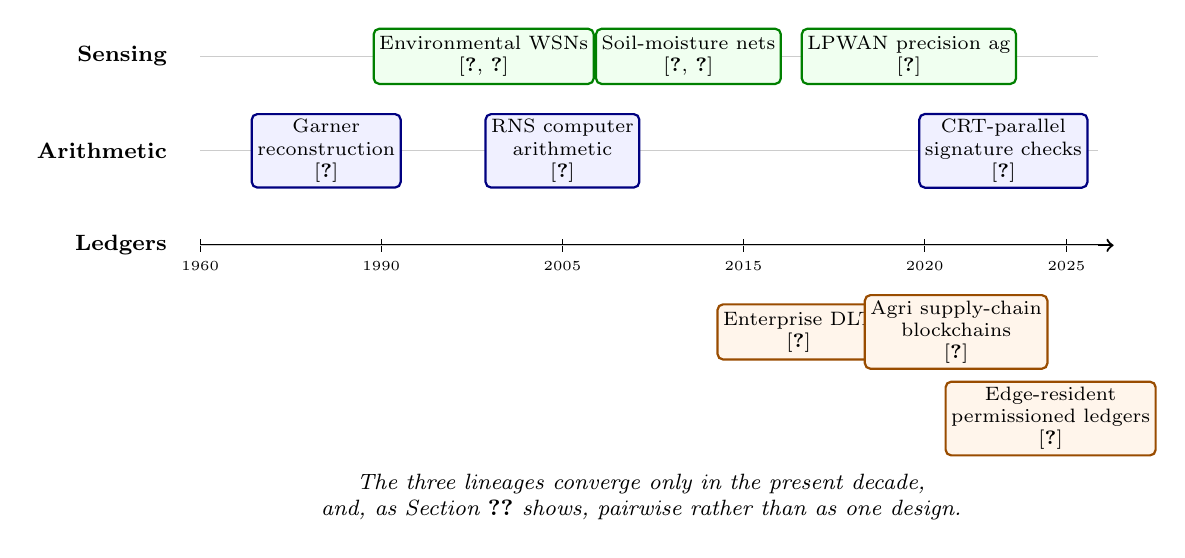
\begin{tikzpicture}[
      lane/.style={font=\footnotesize\bfseries},
      seg/.style={draw, thick, rounded corners=2pt, minimum height=7mm,
                  align=center, font=\scriptsize, inner sep=2pt},
      yr/.style={font=\tiny, align=center}
    ]
\draw[->, thick] (0,0) -- (11.6,0) node[right, font=\footnotesize]{};
    \foreach \x/\lab in {0/1960, 2.3/1990, 4.6/2005, 6.9/2015, 9.2/2020, 11/2025}
      \draw (\x,0.08) -- (\x,-0.08) node[below, yr]{\lab};

\node[lane, anchor=east] at (-0.3,2.4) {Sensing};
    \draw[gray!40, thin] (0,2.4) -- (11.4,2.4);
    \node[seg, fill=green!6, draw=green!50!black] at (3.6,2.4)
      {Environmental WSNs\\\cite{wang2006wireless,pierce1999site}};
    \node[seg, fill=green!6, draw=green!50!black] at (6.2,2.4)
      {Soil-moisture nets\\\cite{bogena2010soil,evans2008precision}};
    \node[seg, fill=green!6, draw=green!50!black] at (9.0,2.4)
      {LPWAN precision ag\\\cite{adelantado2017understanding}};

\node[lane, anchor=east] at (-0.3,1.2) {Arithmetic};
    \draw[gray!40, thin] (0,1.2) -- (11.4,1.2);
    \node[seg, fill=blue!6, draw=blue!50!black] at (1.6,1.2)
      {Garner\\reconstruction\\\cite{garner1959residue}};
    \node[seg, fill=blue!6, draw=blue!50!black] at (4.6,1.2)
      {RNS computer\\arithmetic\\\cite{ding1996remainder}};
    \node[seg, fill=blue!6, draw=blue!50!black] at (10.2,1.2)
      {CRT-parallel\\signature checks\\\cite{beloa2025bitcoincrt}};

\node[lane, anchor=east] at (-0.3,0) {Ledgers};
    \draw[gray!40, thin] (0,0) -- (11.4,0.0);
    \node[seg, fill=orange!8, draw=orange!60!black] at (7.6,-1.1)
      {Enterprise DLT\\\cite{christidis2016blockchain}};
    \node[seg, fill=orange!8, draw=orange!60!black] at (9.6,-1.1)
      {Agri supply-chain\\blockchains\\\cite{tian2016agri}};
    \node[seg, fill=orange!8, draw=orange!60!black] at (10.8,-2.2)
      {Edge-resident\\permissioned ledgers\\\cite{tar2023fabric}};

    \node[font=\footnotesize\itshape, align=center] at (5.6,-3.2)
      {The three lineages converge only in the present decade,\\
       and, as Section~\ref{sec:lit_specific} shows, pairwise rather than as one design.};
  \end{tikzpicture}
  \caption{Three lineages of literature underlying this thesis: agricultural
           sensing, residue arithmetic, and distributed ledgers. Each
           developed largely independently for decades before beginning to
           intersect in the 2020s.}
  \label{fig:lit-timeline}
\end{figure}

\section{The Theory and Research Literature Specific to the Topic}
\label{sec:lit_specific}

\subsection{Precision Agriculture and Internet of Things Sensing}
\label{subsec:lit_precision_ag}

Precision agriculture research has consistently found that sensing density
and irrigation efficiency move together. \gls{iot} soil and canopy sensing
networks demonstrated early that automated, sensor-driven scheduling
outperforms calendar-based irrigation on both water use and
yield~\cite{rathi2025smart, brooks2019precisionWater, chatterjee2023precision,
gondchawar2016agriculture4}, a finding replicated across arid and
semi-arid contexts where the water-saving incentive is
largest~\cite{williams2022savings, miller2020climateImpact,
garrido2018mediterranean}. Reviews of the field converge on the same three
limitations. First, decision-support integration remains
fragmented: sensor data reaches a dashboard but rarely a closed-loop
controller with an auditable
rationale~\cite{aydin2021comprehensive, zhang2002precision,
gebbers2010precision, mcbratney2005future}. Second, most systems evaluate
the analytics rather than the network that feeds them, so machine-learning
yield and stress models are reported against clean, simulated input streams
rather than the loss and jitter that a field deployment actually
produces~\cite{chlingaryan2018machine, goap2018iot, mohanty2016using,
van2020review}. Third, sensing accuracy in the field degrades in ways a
laboratory calibration does not capture, drift, fouling and intermittent
failure among them, and few studies report the resulting error
budget~\cite{akhtar2019sensingAccuracy, agri2024sensorAccuracy,
garcia2021sensorFailures, lopez2023remoteFailure}. Later generations of this
literature push toward higher automation, describing four- and
five-generation smart-farming stacks that assume the identity and integrity
of every reading rather than establishing
it~\cite{suleiman2025agriculture5, owusu2025iotAgri, yang2021iotSensing,
singh2019iotSmartIrrigation, jin2025productivity}. That assumption is exactly
the gap Section~\ref{subsec:lit_blockchain_ag} returns to.

\subsection{Low-Power Wide-Area Network Transmission Optimisation and Energy
Modelling}
\label{subsec:lit_lpwan}

\gls{lora} is the dominant physical layer in this literature because it
reaches farm-scale distances, of the order of kilometres in rural terrain,
from a battery node at sub-milliwatt receive
power~\cite{raza2018lorawan, li2020performance, raj2017comprehensive}. The
cost is airtime. The Semtech chirp spread-spectrum design fixes the time to
transmit a payload of $PL$ bytes as a function of spreading factor $\mathrm{SF}$,
bandwidth $\mathrm{BW}$, coding rate $\mathrm{CR}$ and the low-data-rate
optimisation flag $\mathrm{DE}$~\cite{semtech2015lorawan, bor2016lorawan}.
The symbol period is
\begin{equation}
T_{\text{sym}} = \frac{2^{\mathrm{SF}}}{\mathrm{BW}},
\label{eq:lora_symbol}
\end{equation}
the payload requires
\begin{equation}
n_{\text{payload}} = 8 + \max\!\left(
  \left\lceil \frac{8\,PL - 4\,\mathrm{SF} + 28 + 16\,\mathrm{CRC} - 20\,\mathrm{IH}}
                    {4(\mathrm{SF} - 2\,\mathrm{DE})} \right\rceil
  (\mathrm{CR}+4),\; 0 \right)
\label{eq:lora_payload_symbols}
\end{equation}
symbols, and total airtime is
\begin{equation}
T_{\text{air}} = \underbrace{(n_{\text{preamble}} + 4.25)\, T_{\text{sym}}}_{\text{preamble}}
               + n_{\text{payload}} \, T_{\text{sym}}.
\label{eq:lora_airtime}
\end{equation}
Equation~\ref{eq:lora_airtime} is the quantity every optimisation in this
literature ultimately reduces: for a fixed $\mathrm{SF}$ and $\mathrm{BW}$,
airtime is affine in payload length, so a shorter payload is the only lever
available once the modulation is chosen. Regulatory duty-cycle limits then
convert that airtime into a rate ceiling rather than merely an energy cost.
Under \gls{etsi} EN\,300\,220, a sub-GHz node may occupy its channel for at
most a fixed fraction $\mathrm{DC}_{\max}$ of any observation
window~\cite{ttn2024eu868, loraalliance2021regional}, so a single reading
consumes
\begin{equation}
\mathrm{DC} = \frac{T_{\text{air}}}{T_{\text{window}}} \leq \mathrm{DC}_{\max},
\label{eq:duty_cycle}
\end{equation}
and offered channel load across $N$ nodes reporting once per window is
$G = N\,T_{\text{air}}/T_{\text{window}}$ Erlang, which under the pure-ALOHA
assumption common to this literature bounds per-packet collision probability
at $P_{\text{coll}} = 1 - e^{-2G} \approx 2G$ for small
$G$~\cite{bor2016lorawan, adelantado2017understanding}. Node energy per
transmission follows directly, $E_{\text{tx}} = P_{\text{tx}}\,T_{\text{air}}$,
so any reduction in $T_{\text{air}}$ is simultaneously an energy saving and a
capacity gain, which is why the transmission-optimisation literature and the
energy-modelling literature are, in practice, one
body of work~\cite{barr1994energy, polastre2005versatile, gonzalez2000energy,
mohammed2025loraEnergy, sanchez2021energy, heinzelman2000energy}.

Two families of technique attack Equation~\ref{eq:lora_airtime} from
opposite sides, summarised in Figure~\ref{fig:lit-transmission-taxonomy}.
\textbf{Compression} keeps one packet per reading and shrinks $PL$: general
lossless coders such as Huffman and Lempel-Ziv-Welch adapted to sensor
streams~\cite{li2018lossless, marcelloni2009energy, ziv1977universal,
huffman1952method, salomon2007data} report 20 to 40\% payload reduction but
require dictionary or frequency-table state that a microcontroller with a
few kilobytes of free \gls{ram} can only marginally
afford~\cite{chen2025compression, lzw_dictionary_size}, and adaptive
sampling reduces transmitted volume by skipping readings, which risks
missing the threshold event the network exists to
detect~\cite{kjellsson2008adaptive}. \textbf{Decomposition} takes the
opposite path: it accepts more packets in exchange for each one being
far shorter, splitting a reading across parallel channels rather than
compressing it on one. Residue-based decomposition for wireless sensor
data has been explored for storage reduction and for wireless sensor
network lifetime~\cite{vidhya2021crt, crtcompression2018, khan2023fuzzycrt,
rahman2022rnsenergy, djeddi2025parallelCRT}, but, as
Section~\ref{subsec:lit_crt} details, not for exploiting a multi-channel
concentrator's ability to demodulate several sub-channels
\emph{simultaneously}, which is the specific mechanism this thesis studies.
LoRa-specific network-capacity work independently confirms that channel
occupancy, not raw byte count, is the binding constraint on
gateway-served node population~\cite{centenaro2016lorawanlimits,
zhang2022lorawan, chapungo2025lorawan, bicamumakuba2025lorawan,
turlykozhayeva2024proactive, mozambique2021lorawan}, which is the same
quantity Equation~\ref{eq:duty_cycle} fixes.

\begin{figure}[htbp]
  \centering
  \begin{tikzpicture}[
      root/.style={draw, thick, rounded corners=2pt, fill=black!5,
                   font=\small\bfseries, align=center, minimum width=42mm,
                   minimum height=8mm},
      branch/.style={draw, rounded corners=2pt, font=\footnotesize\bfseries,
                     align=center, minimum width=38mm, minimum height=8mm},
      leaf/.style={draw, rounded corners=2pt, font=\scriptsize, align=center,
                   text width=30mm, minimum height=11mm, inner sep=2pt},
      e/.style={-{Stealth[length=1.8mm]}, thick, draw=black!60}
    ]
    \node[root] (r) at (0,4.4) {Reduce airtime\\$T_{\text{air}}$ (Eq.~\ref{eq:lora_airtime})};

    \node[branch, fill=red!6, draw=red!55!black] (c) at (-4.2,2.6) {Compression\\(one packet)};
    \node[branch, fill=blue!6, draw=blue!55!black] (d) at (4.2,2.6) {Decomposition\\(many packets)};
    \draw[e] (r.south) -- ++(0,-0.4) -| (c.north);
    \draw[e] (r.south) -- ++(0,-0.4) -| (d.north);

    \node[leaf, fill=red!4] (c1) at (-6.0,0.6) {Dictionary coders\\(LZW, Huffman)\\\cite{li2018lossless,marcelloni2009energy}};
    \node[leaf, fill=red!4] (c2) at (-2.4,0.6) {Adaptive\\sampling\\\cite{kjellsson2008adaptive}};
    \draw[e] (c.south) -- ++(0,-0.4) -| (c1.north);
    \draw[e] (c.south) -- ++(0,-0.4) -| (c2.north);

    \node[leaf, fill=blue!4] (d1) at (2.4,0.6) {Residue storage\\\ \& lifetime\\\cite{vidhya2021crt,rahman2022rnsenergy}};
    \node[leaf, fill=blue!4] (d2) at (6.0,0.6) {Multi-channel\\parallel reception\\(this thesis)};
    \draw[e] (d.south) -- ++(0,-0.4) -| (d1.north);
    \draw[e] (d.south) -- ++(0,-0.4) -| (d2.north);

    \node[font=\footnotesize\itshape, text width=105mm, align=center] at (0,-1.7)
      {Compression shrinks the payload on one channel; decomposition trades
       packet count for per-packet occupancy across several. The literature
       has developed the left branch thoroughly and the right branch for
       storage and lifetime, but not yet for concurrent multi-channel
       reception.};
  \end{tikzpicture}
  \caption{Taxonomy of transmission-efficiency strategies for constrained
           \gls{iot} radios. This thesis occupies the shaded leaf on the
           right that the reviewed literature leaves open.}
  \label{fig:lit-transmission-taxonomy}
\end{figure}

Table~\ref{tab:lit-lpwan-comparison} summarises representative results
across both branches on the metric that matters for gateway capacity,
per-packet airtime or its energy equivalent, rather than the compression
ratio each source reports on its own terms.

\begin{table}[htbp]
\centering
\caption{Representative low-power wide-area transmission-efficiency results}
\label{tab:lit-lpwan-comparison}
\footnotesize
\begin{tabularx}{\textwidth}{@{}p{0.21\textwidth}p{0.18\textwidth}X@{}}
\toprule
\textbf{Study} & \textbf{Technique} & \textbf{Reported limitation} \\
\midrule
Li and Simonot-Lion~\cite{li2018lossless};\\ Marcelloni and Vecchio~\cite{marcelloni2009energy}
  & Huffman/LZW sensor compression
  & Dictionary or frequency-table state exceeds the free \gls{ram} of the
    smallest microcontroller class; ratio degrades on low-entropy sensor
    streams \\
\midrule
Kjellsson et al.~\cite{kjellsson2008adaptive}
  & Adaptive, event-driven sampling
  & Reduces volume, not per-packet occupancy; risks missing threshold
    events between samples \\
\midrule
Vidhya and Brindha~\cite{vidhya2021crt,crtcompression2018}
  & \gls{crt} residue image compression
  & Targets storage footprint, not transmission concurrency; single-channel
    model \\
\midrule
Buttigieg et al.~\cite{khan2023fuzzycrt};\\ Pourbigharaz and Yassine~\cite{rahman2022rnsenergy}
  & \gls{rns} energy reduction in \glspl{wsn}
  & Energy accounting only; no gateway-capacity or multi-channel reception
    model \\
\midrule
Ye et al.~\cite{djeddi2025parallelCRT}
  & \gls{rns}-based reliable \gls{wsn} transmission
  & Reliability under loss, not concurrent channel exploitation \\
\bottomrule
\end{tabularx}
\end{table}

\subsection{Residue Number Systems and the Chinese Remainder Theorem in
Communications}
\label{subsec:lit_crt}

The theorem itself is unconditional. For pairwise coprime moduli
$m_1,\ldots,m_k$ and $M = \prod_{i=1}^{k} m_i$, every integer
$x \in [0,M)$ is uniquely determined by its residue vector
$(r_1,\ldots,r_k)$, $r_i = x \bmod m_i$~\cite{garner1959residue,
hardy2008introduction}. Garner's algorithm reconstructs $x$ from the
residues in closed form,
\begin{equation}
x = \left( \sum_{i=1}^{k} r_i\, M_i\, N_i \right) \bmod M, \qquad
M_i = \frac{M}{m_i}, \quad N_i = M_i^{-1} \bmod m_i,
\label{eq:crt_reconstruction}
\end{equation}
exact because $M_i N_i \equiv 1 \pmod{m_i}$ by
construction~\cite{garner1959residue, knuth1997art}, and computable in
$O(k)$ modular multiplications regardless of the magnitude of $x$, which is
the property that later work in residue number systems generalised into a
programme for fast, carry-free, parallel
arithmetic~\cite{ding1996remainder, parhami2010computer}. A second
property of Equation~\ref{eq:crt_reconstruction} bears on reliability
rather than speed. Goldreich, Ron and Sudan formalised the error-tolerant
case, showing that $x$ remains recoverable from a strict subset of
residues under bounded corruption, "Chinese remaindering with
errors"~\cite{goldreich1999china}, a result later systematised alongside
subset-product reconstruction in computational number
theory~\cite{shoup2009computational}. That subset-recovery property is a
statement about \emph{reconstruction}, not about \emph{disclosure}: it is
tempting to read a residue set as a threshold secret-sharing scheme, exact
recovery from a complete or near-complete subset, negligible information
from any one share in isolation, but the two constructions are not
equivalent. A Shamir-style share is deliberately randomised so that any
share short of the threshold is uniformly distributed independent of the
secret~\cite{shoup2009computational}; a plain \gls{crt} residue is not.
$r_i = x \bmod m_i$ is a deterministic function of $x$, so intercepting it
narrows the field of possible values by a factor of roughly $m_i$ rather
than leaking nothing, and if the plaintext domain is itself small relative
to $m_i$, a single residue can narrow that field to very little uncertainty
indeed. Whether residue disclosure is negligible in practice therefore
depends on the ratio between the plaintext's domain and the moduli chosen,
not on the reconstruction identity alone, and the reviewed literature has
not established that ratio for any deployed system;
Section~\ref{subsec:lit_privacy} returns to this distinction, and Chapter
One's hypothesis H5 treats it as open rather than established.

Three application communities have used
Equations~\ref{eq:crt_reconstruction} for three different resources. The
first treats it as a \emph{storage} problem: residue-based lossless image
compression reports 15 to 30\% footprint reduction with exact
reconstruction~\cite{vidhya2021crt, crtcompression2018}. The second treats
it as an \emph{energy} problem inside wireless sensor
networks, converting a single wide-range reading into several
narrow-range residues to shrink the arithmetic and storage cost per
node~\cite{rahman2022rnsenergy, khan2023fuzzycrt, djeddi2025parallelCRT}.
The third, established in the candidate's own prior
work~\cite{beloa2025bitcoincrt}, treats it as a \emph{processor-cycle}
problem: decomposing the modular exponentiation inside \gls{ecdsa}
signature verification into $k$ independent sub-computations over smaller
coprime moduli, each assignable to a separate core, so that Bitcoin
transaction validation throughput increases without a change to block size
or consensus rules. That result establishes the arithmetic and the
parallelisation argument at the centre of a blockchain node; it does not
address the constrained radio link at the edge of a sensor network, where
the scarce resource is airtime rather than \gls{cpu} cycles, nor the
identity and confidentiality questions that arise once residues cross a
shared wireless medium rather than staying inside one machine's memory.
Figure~\ref{fig:lit-crt-pipelines} sets the two pipelines side by side.
This thesis takes the arithmetic of Equation~\ref{eq:crt_reconstruction} as
established by all three communities and asks what it is worth when the
parallel resource is a multi-channel radio concentrator rather than a
multi-core processor, which, to the reviewed literature's knowledge, no
prior system has done~\cite{wang2018novel}.

\begin{figure}[htbp]
  \centering
  \begin{tikzpicture}[
      stg/.style={draw, rounded corners=2pt, align=center, font=\scriptsize,
                  minimum height=8mm, minimum width=24mm, inner sep=2pt},
      e/.style={-{Stealth[length=1.8mm]}, thick},
      lbl/.style={font=\footnotesize\bfseries}
    ]
    \node[lbl] at (-5.4,3.0) {Prior work~\cite{beloa2025bitcoincrt}:};
    \node[stg, fill=blue!6, draw=blue!55!black] (v1) at (-4.4,1.6) {Value $x$\\(signature field)};
    \node[stg, fill=blue!6, draw=blue!55!black] (r1) at (-1.6,1.6) {Residues\\$r_1,\ldots,r_k$};
    \node[stg, fill=blue!6, draw=blue!55!black] (p1) at (1.2,1.6) {$k$ CPU cores\\(parallel)};
    \node[stg, fill=blue!6, draw=blue!55!black] (x1) at (4.0,1.6) {Reconstructed\\signature check};
    \draw[e] (v1) -- (r1); \draw[e] (r1) -- (p1); \draw[e] (p1) -- (x1);
    \node[font=\scriptsize\itshape] at (-1.6,0.75) {Eq.~\ref{eq:crt_reconstruction} applied inside one machine};

    \node[lbl] at (-5.1,-0.9) {This thesis:};
    \node[stg, fill=green!6, draw=green!50!black] (v2) at (-4.4,-2.3) {Value $x$\\(sensor reading)};
    \node[stg, fill=green!6, draw=green!50!black] (r2) at (-1.6,-2.3) {Residues\\$r_1,\ldots,r_k$};
    \node[stg, fill=green!6, draw=green!50!black] (p2) at (1.2,-2.3) {$k$ radio\\sub-channels};
    \node[stg, fill=green!6, draw=green!50!black] (x2) at (4.0,-2.3) {Reconstructed\\reading at gateway};
    \draw[e] (v2) -- (r2); \draw[e] (r2) -- (p2); \draw[e] (p2) -- (x2);
    \node[font=\scriptsize\itshape] at (-1.6,-3.15) {Eq.~\ref{eq:crt_reconstruction} applied across a shared wireless medium};
  \end{tikzpicture}
  \caption{The same reconstruction identity (Eq.~\ref{eq:crt_reconstruction})
           applied to two different parallel resources. Prior work
           parallelises processor cycles inside one machine; this thesis
           parallelises radio sub-channels across a shared medium, which
           introduces identity and confidentiality questions the prior
           application does not face.}
  \label{fig:lit-crt-pipelines}
\end{figure}

\subsection{Blockchain and Distributed Ledger Technology in Agriculture and
Supply Chains}
\label{subsec:lit_blockchain_ag}

A distributed ledger's tamper evidence rests on hash chaining: each block
$B_i$ commits to its predecessor and its own transaction set through
\begin{equation}
h_i = H\!\left( h_{i-1} \,\|\, \mathrm{tx}_i \right),
\label{eq:hash_chain}
\end{equation}
where $H$ is a cryptographic hash function, so that altering any committed
$\mathrm{tx}_j$ for $j \le i$ requires recomputing every $h_j,\ldots,h_i$
across every replica that holds the chain, a cost that grows with the
number of mutually distrusting replicas rather than
shrinking~\cite{fernandez2024iotTamper}. Merkle's original construction
generalises Equation~\ref{eq:hash_chain} to a binary tree of hashes so that
membership of a single transaction can be proven in $O(\log n)$ rather than
by revealing the whole block, a property later systems use for compact
audit proofs~\cite{sharma2018merkle}. Applied to agriculture, this
tamper-evidence property has been used for supply-chain
transparency~\cite{tian2016agri, kamilaris2019rise, oh2025foodsafety,
galvez2018future, tian2017traceability, reyna2018blockchain, tian2017agri,
kamilaris2018food}, farm-data
management~\cite{lin2018blockchain, ferrag2020security, haque2024scalable,
zhang2019blockchain, aliyu2023blockchainbasedsmartfarm}, and smart-contract
automation of certification and payment
logic~\cite{rama2021systematic, patil2022blockchain, nguyen2022smartFarmingSC,
ahmad2025agriBlockchain, zhu2017blockchainAgri}. Cross-organisational data
sharing has more recently been framed through self-sovereign identity,
letting a farm operator authorise fine-grained access without handing a
consortium a standing credential~\cite{amraouy2025ssi}, and water-quality
and irrigation-specific ledgers report similar tamper-evidence
gains~\cite{saito2025blockchainWaterQuality, liu2024blockchainwater,
arshad2022blockchainBenefits, ali2023farmDataTampering,
rahman2019agriSecurity}. The generic \gls{iot}-blockchain integration
literature that agricultural systems draw their architecture from
independently confirms the same design pattern: a lightweight device signs
and forwards, a gateway or edge node validates and submits, and the ledger
anchors a hash rather than the raw
payload~\cite{dorri2017blockchain, nguyen2019blockchain, xu2020making,
reyna2018blockchain, benedict2021decentralized}.

What this body of literature does not establish is where the tamper
evidence begins. Almost every system surveyed authenticates at the gateway
or the enterprise boundary and treats the sensor as an untrusted data
source whose values are accepted once they arrive, not a principal whose
identity is bound to the record it produced~\cite{lin2020blockchain,
ferrag2020blockchain, xu2019survey, george2025review,
pereira2023blockchainTrust}. Table~\ref{tab:lit-blockchain-ag} makes this
concrete across a representative sample: the column that is consistently
weak or absent is node-level, rather than gateway-level, identity binding,
which is precisely the gap Chapter One's problem statement
(Section~\ref{sec:problem}) identifies.

\begin{table}[htbp]
\centering
\caption{Representative blockchain-in-agriculture systems by authentication
         boundary and evaluation setting}
\label{tab:lit-blockchain-ag}
\footnotesize
\begin{tabularx}{\textwidth}{@{}p{0.24\textwidth}p{0.19\textwidth}p{0.16\textwidth}X@{}}
\toprule
\textbf{Study} & \textbf{Authentication boundary} & \textbf{Evaluation setting} & \textbf{Reported gap} \\
\midrule
Tian~\cite{tian2016agri}; Kamilaris et al.~\cite{kamilaris2019rise}
  & Enterprise / consortium & Conceptual, no field data
  & No per-sensor identity; throughput not characterised on constrained hardware \\
\midrule
Zhang et al.~\cite{zhang2019blockchain}
  & Gateway & Simulation
  & Consensus cost assumed server-class hardware \\
\midrule
Amraouy et al.~\cite{amraouy2025ssi}
  & Farm operator (self-sovereign identity)
  & Prototype
  & Access-sharing framework; no edge-hardware performance data \\
\midrule
Reyna et al.~\cite{reyna2018blockchain}; Dorri et al.~\cite{dorri2017blockchain}
  & Generic \gls{iot} gateway & Survey / architecture
  & Identifies the sensor-to-gateway trust gap without closing it \\
\bottomrule
\end{tabularx}
\end{table}

\subsection{Edge-Resident Consensus and Constrained-Hardware Ledgers}
\label{subsec:lit_consensus}

Running a permissioned ledger on gateway-class hardware raises a question
the enterprise blockchain literature rarely poses: whether consensus can
complete inside the timing budget of a real-time control loop, on a device
with an order of magnitude less memory and \gls{cpu} throughput than the
server hardware that literature assumes~\cite{tar2023fabric,
jayaram2023hyperledger, ibmFabric}. Hyperledger Fabric's execute-order-validate
architecture separates transaction endorsement from ordering, letting an
ordering service reach agreement on transaction sequence rather than
transaction content, and the Raft ordering service used in this thesis
implements crash-fault-tolerant, not Byzantine-fault-tolerant,
agreement~\cite{ongaro2014raft, orderingServiceDoc}. The distinction has a
direct complexity consequence. \gls{cft} protocols such as Raft reach
agreement with $O(n)$ message exchanges per decision and tolerate
$f = \lfloor (n-1)/2 \rfloor$ stopped nodes, whereas classical
\gls{bft} protocols such as \gls{pbft} require $n \geq 3f+1$ replicas,
so they tolerate the smaller
$f = \lfloor (n-1)/3 \rfloor$, at $O(n^2)$ messages per decision, to
withstand arbitrary, not merely crash, node
behaviour~\cite{castro1999practical, ongaro2014raft}. A five-node
cluster therefore tolerates two stopped nodes under Raft but only one
Byzantine node under \gls{pbft}, a smaller fault budget bought at a
quadratically larger message cost. Linear-complexity \gls{bft} variants
such as HotStuff
close much of that gap for adversarial settings~\cite{yin2019hotstuff}, and
the state-machine-replication literature more broadly treats the
\gls{cft}/\gls{bft} choice as a trade between message cost and the
threat model tolerated~\cite{bessani2014state}. This thesis, deployed on a
consortium of trusted, physically secured gateways rather than an open or
adversarial network, adopts \gls{cft} for that reason, a choice the
consensus literature supports for permissioned agricultural
settings~\cite{dube2024fabricIrrigation} but rarely evaluates on
gateway-class \gls{arm64} hardware in the field, as
Table~\ref{tab:lit-consensus} shows.

\begin{figure}[htbp]
  \centering
  \begin{tikzpicture}[
      root/.style={draw, thick, rounded corners=2pt, fill=black!5, font=\small\bfseries,
                   align=center, minimum width=46mm, minimum height=8mm},
      branch/.style={draw, rounded corners=2pt, font=\footnotesize\bfseries,
                     align=center, minimum width=40mm, minimum height=8mm},
      leaf/.style={draw, rounded corners=2pt, font=\scriptsize, align=center,
                   text width=34mm, minimum height=13mm, inner sep=2pt},
      e/.style={-{Stealth[length=1.8mm]}, thick, draw=black!60}
    ]
    \node[root] (r) at (0,4.2) {Fault model tolerated};

    \node[branch, fill=teal!6, draw=teal!55!black] (cft) at (-4.6,2.4) {Crash-fault\\tolerant};
    \node[branch, fill=purple!6, draw=purple!55!black] (bft) at (4.6,2.4) {Byzantine-fault\\tolerant};
    \draw[e] (r.south) -- ++(0,-0.4) -| (cft.north);
    \draw[e] (r.south) -- ++(0,-0.4) -| (bft.north);

    \node[leaf, fill=teal!4] (l1) at (-4.6,0.2)
      {Raft\\$O(n)$ msgs/decision\\$f=\lfloor(n-1)/2\rfloor$\\\cite{ongaro2014raft}\\\emph{used in this thesis}};

    \node[leaf, fill=purple!4] (l2) at (2.2,0.2)
      {\gls{pbft}\\$O(n^2)$ msgs/decision\\$f=\lfloor(n-1)/3\rfloor$\\\cite{castro1999practical}};
    \node[leaf, fill=purple!4] (l3) at (7.0,0.2)
      {HotStuff\\$O(n)$ msgs/decision,\\linear view-change\\\cite{yin2019hotstuff}};
    \draw[e] (bft.south) -- ++(0,-0.4) -| (l2.north);
    \draw[e] (bft.south) -- ++(0,-0.4) -| (l3.north);

    \node[font=\footnotesize\itshape, text width=110mm, align=center] at (0,-2.0)
      {Message complexity scales with the fault model tolerated, not with
       hardware class. \gls{cft} is adopted here because the deployment is a
       trusted, physically secured consortium; the reviewed literature
       rarely reports which choice was measured on \gls{arm64} gateway
       hardware rather than assumed server-class hardware.};
  \end{tikzpicture}
  \caption{Consensus fault models and their message complexity, after
           \cite{ongaro2014raft,castro1999practical,yin2019hotstuff,
           bessani2014state}.}
  \label{fig:lit-consensus-taxonomy}
\end{figure}

Whichever protocol is chosen, its saturation behaviour under load is
standard queueing theory. Treating packet or transaction arrivals as
Poisson and service time as deterministic (an M/D/1 queue), mean waiting
time before service is
\begin{equation}
W_q = \frac{\rho}{2(1-\rho)}\, T_{\text{service}}, \qquad
\rho = \lambda\, T_{\text{service}},
\label{eq:mdOne}
\end{equation}
where $\lambda$ is the arrival rate and $T_{\text{service}}$ the
deterministic service time, so that total latency $L = T_{\text{service}} +
W_q$ is flat while $\rho \ll 1$ and diverges as $\rho \to 1$. The
scalability literature for both LoRa gateways and blockchain orderers uses
Equation~\ref{eq:mdOne}, or its close relatives, to project a saturation
point from a small deployment rather than requiring one at
scale~\cite{fabric2019performance, pinto2024throughput, cui2023ipfsFabric,
rahimi2023fabricSensors, khan2021fabricCRT}, but, as with the consensus
literature above, validation against real field load rather than synthetic
benchmark load remains the exception rather than the
rule. The \gls{cap} theorem underlies the same trade from a different
angle: no distributed data store can simultaneously guarantee consistency
and availability under network partition~\cite{brewer2000towards,
gilbert2002brewer}, and permissioned ledgers on intermittently connected
rural gateways sit squarely inside that trade-off, a point the
practitioner literature on eventual, \gls{acid}-relaxed consistency in
distributed systems makes explicit~\cite{pritchett2008base}.

\begin{table}[htbp]
\centering
\caption{Consensus and edge-ledger literature by hardware class evaluated}
\label{tab:lit-consensus}
\footnotesize
\begin{tabularx}{\textwidth}{@{}p{0.22\textwidth}p{0.18\textwidth}p{0.14\textwidth}X@{}}
\toprule
\textbf{Study} & \textbf{Protocol} & \textbf{Hardware class} & \textbf{Reported gap} \\
\midrule
Ongaro and Ousterhout~\cite{ongaro2014raft}
  & Raft (\gls{cft})
  & Server-class (original)
  & Correctness and understandability proof; no constrained-hardware
    evaluation \\
\midrule
Castro and Liskov~\cite{castro1999practical}
  & \gls{pbft} (\gls{bft})
  & Server-class
  & $O(n^2)$ messaging cost not evaluated against gateway bandwidth \\
\midrule
Androulaki et al.~\cite{jayaram2023hyperledger}
  & Fabric E-O-V pipeline
  & Data-centre reference deployment
  & Throughput figures not reproduced on \gls{arm64} \\
\midrule
Rahimi et al.~\cite{rahimi2023fabricSensors}; Cui et al.~\cite{cui2023ipfsFabric}
  & Fabric + sensor / off-chain storage
  & Prototype, short-duration
  & No sustained field deployment; saturation point not field-validated \\
\bottomrule
\end{tabularx}
\end{table}

\subsection{Identity, Access Control and Privacy-Preserving Data Processing}
\label{subsec:lit_privacy}

Two threads meet here: how a permissioned ledger decides who may act, and
how it protects what a record discloses to parties who are entitled to see
that it exists but not what it contains. On the first thread, \gls{rbac}
enforced in chaincode is the standard mechanism, with permissions attached
to roles rather than individual identities and a \gls{msp} resolving each
transaction's submitter to a role through its
\gls{x509} certificate~\cite{mdpiAccessControl, hyperledger2022msp}. The
candidate's own prior formalisation of this
mechanism~\cite{beloasone2025hrbac} extends flat \gls{rbac} with a role
hierarchy expressed as a partial order $\preceq$ over the role set $R$,
where $r_i \preceq r_j$ iff $\mathrm{permissions}(r_i) \subseteq
\mathrm{permissions}(r_j)$, so that a user $u$'s effective permission set
in a session is the union across every role dominated by an active role,
\begin{equation}
\mathrm{eff}(u) = \bigcup_{r \in \mathrm{active}(u)} \; \bigcup_{r' \preceq r} pa(r'),
\label{eq:hrbac_eff}
\end{equation}
with $pa(r)$ the permissions directly assigned to role $r$. An access
request $(u, op, res, t)$ is then granted only if an active, non-expired
role of $u$ carries the requested permission \emph{and} the requester's
zone matches the resource's zone or the requester holds an
administrator-issued cross-zone token,
\begin{equation}
\exists\, r \in \mathrm{active}(u,t) : (op,res) \in \mathrm{eff}(r)
\;\land\; \bigl(\mathrm{zone}(u) = \mathrm{zone}(res) \lor
\mathrm{czt}(u,\mathrm{zone}(res),t)\bigr),
\label{eq:hrbac_grant}
\end{equation}
which folds zone and temporal constraints directly into the access
decision rather than leaving them to an external policy
layer~\cite{beloasone2025hrbac}. This formalisation follows the general
tradition of administrative role hierarchies in access-control
theory~\cite{lu2022revocation} and shares its enforcement point, the
chaincode's client-identity check, with the wider Fabric access-control
literature~\cite{mdpiAccessControl}, but it authenticates at the
\emph{gateway}, the device holding the \gls{x509} certificate that signs
the transaction, not at the individual sensing node whose reading the
transaction carries. Certificate revocation latency under this model has
been measured directly, with propagation delay across a small
gossip-connected peer set on the order of minutes rather than
seconds~\cite{lu2022revocation}, a figure this thesis's own deployment
reproduces independently rather than merely assumes.

On the second thread, privacy in a replicated ledger is structurally
difficult: the same replication that gives every consortium member a
tamper-evident copy of a record also gives every member a copy of whatever
that record discloses. Off-chain storage with an on-chain hash anchor is
the common mitigation, verifiable without being
world-readable~\cite{kim2023privacy}, and self-sovereign identity schemes
extend the same principle to access itself, letting a data owner grant and
revoke visibility without a standing
credential~\cite{amraouy2025ssi}. Neither line of work, however, asks
whether the transmission layer itself can contribute to confidentiality
before a record ever reaches the ledger. Section~\ref{subsec:lit_crt}
showed why that question is harder than it first looks: reconstruction
tolerates a missing residue under Goldreich, Ron and Sudan's
error-tolerant formulation~\cite{goldreich1999china}, but a plain
\gls{crt} residue is not a randomised secret share, so subset-recovery
tolerance does not, by itself, establish subset-disclosure
resistance~\cite{shoup2009computational}. What it establishes instead is
a precise condition worth testing rather than assuming: disclosure from
an intercepted residue is bounded by how far the plaintext's domain
exceeds the missing moduli's product, so confidentiality is a property of
the deployed moduli-to-domain ratio, not of the reconstruction identity
in the abstract. The literature reviewed here has developed residue
decomposition and threshold secret sharing in separate communities
without stating that condition, which is exactly why Chapter One frames
it as hypothesis H5 rather than a settled result: the rationale
(Section~\ref{sec:rationale}) proposes residue decomposition as a
candidate confidentiality substrate, and H5 requires either a quantified
leakage bound for the deployed moduli and sensor ranges, or an added
randomisation step, before the substrate can be called established.

\subsection{The Corpus Underlying This Review}
\label{subsec:lit_corpus}

The review draws on a corpus of 120 full-text papers assembled by systematic
retrieval against the reference lists of the source manuscripts and by
open-access topic search around the five themes above. Table~\ref{tab:corpus}
records its composition, and Figure~\ref{fig:corpus-year} its distribution over
time.

\begin{table}[htbp]
  \centering
  \caption{Composition of the 120-paper corpus by provenance and theme.}
  \label{tab:corpus}
  \begin{singlespace}
  \small
  \begin{tabular}{@{}p{5.6cm}r@{\hskip 12mm}p{4.6cm}r@{}}
    \toprule
    \textbf{Provenance} & \textbf{n} & \textbf{Theme} & \textbf{n} \\
    \midrule
    Open-access topic search        & 44 & Agriculture, supply chain   & 27 \\
    Cited in the reference list     & 35 & Security, identity, privacy & 22 \\
    Prior related work              & 21 & IoT, LoRa, edge computing   & 14 \\
    Cited in the source manuscripts & 20 & Blockchain scalability      & 13 \\
                                    &    & Machine learning            & 11 \\
                                    &    & CRT and residue systems     &  5 \\
                                    &    & Cross-cutting or other      & 28 \\
    \midrule
    \textbf{Total}                  & \textbf{120} & \textbf{Total}     & \textbf{120} \\
    \bottomrule
  \end{tabular}
  \end{singlespace}
\end{table}

\begin{figure}[htbp]
  \centering
  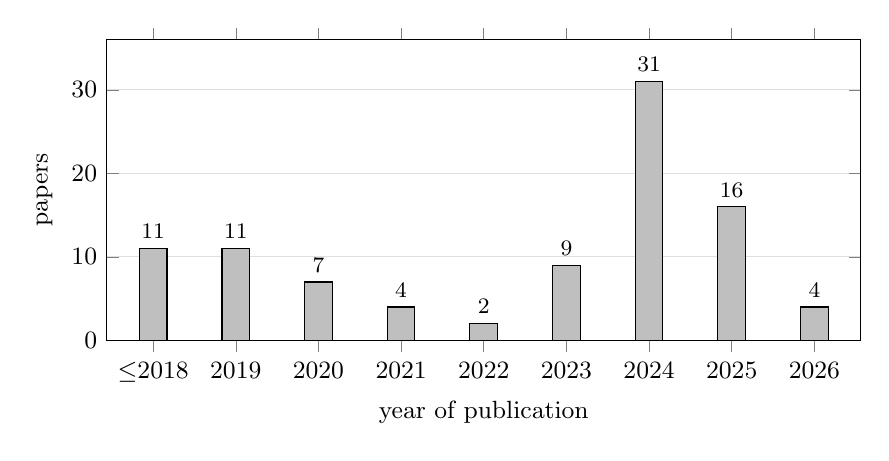
\begin{tikzpicture}
    \begin{axis}[
        ybar, width=0.92\textwidth, height=5.4cm, bar width=10pt,
        ylabel={papers}, xlabel={year of publication},
        xtick={2018,2019,2020,2021,2022,2023,2024,2025,2026},
        xticklabels={$\leq$2018,2019,2020,2021,2022,2023,2024,2025,2026},
        ymin=0, ymax=36, enlarge x limits=0.07,
        nodes near coords, nodes near coords style={font=\footnotesize},
        tick label style={font=\small}, label style={font=\small},
        ymajorgrids, grid style={gray!25},
      ]
      \addplot[draw=black, fill=black!25] coordinates {
        (2018,11) (2019,11) (2020,7) (2021,4) (2022,2)
        (2023,9) (2024,31) (2025,16) (2026,4)};
    \end{axis}
  \end{tikzpicture}
  \caption{Publication years of the 120 reviewed papers. Just over half appeared
           from 2024 onward, which is consistent with the observation of
           Section~\ref{sec:lit_history} that the three lineages have only
           recently begun to intersect.}
  \label{fig:corpus-year}
\end{figure}

Two features of the distribution bear on the argument. Fifty-one of the 120
papers, rather more than two fifths, were published in 2024 or later, so the
questions this thesis addresses are being asked now rather than settled. Only
five papers treat residue arithmetic directly, against 27 on agricultural and
supply-chain applications and 22 on security, identity and privacy. The
arithmetic is the sparsest of the five strands and the least connected to the
others, which is the imbalance the present work exploits.

\subsection{Blockchain Scalability and the Parallelism Argument}
\label{subsec:lit_scalability}

A substantial body of recent work attacks ledger throughput directly, and it
matters here because the parallelisation argument this thesis makes for the
radio link was first made for the ledger.

\subsubsection*{a) Partitioning and sharding}

Sharding partitions state and transaction load across sub-committees so that
disjoint transactions commit concurrently. Recent treatments add adaptive
assignment of accounts to shards~\cite{horvath2025assistedsharding} and survey
the cost, chiefly cross-shard coordination, which grows with the fraction of
transactions touching more than one partition~\cite{anonndscalabilitysolutions}.
\textcite{maiwada2024techniquesimprove} and
\textcite{maiwada2025blockchainscalability} analyse Bitcoin throughput under
transaction-adjournment and related scheduling techniques, reporting the
familiar result that raw block-level parallelism is bounded by the
serialisation the consensus protocol imposes. Layer-two constructions move the
work off chain entirely and settle in
aggregate~\cite{patel2023blockchainlayer}, and hierarchical models have been
used to characterise where the resulting systems
saturate~\cite{sadath2024scalabilityperformance}.

\subsubsection*{b) The common structure of these results}

Every one of these mechanisms decomposes a workload into parts that can be
processed independently and recombines the parts afterwards, and in every case
the recombination cost is what bounds the gain. That is precisely the structure
of a residue decomposition, where the recombination is
Equation~\ref{eq:crt_reconstruction} and its cost is $O(k)$, known in advance
and independent of the data. The present work applies the same argument one
layer down, to the radio rather than to the ledger, where the quantity
partitioned is channel occupancy rather than transaction
load~\cite{forcha2026basedparallel}.

\subsection{Residue Arithmetic Beyond Computer Arithmetic}
\label{subsec:lit_crt_extended}

The \gls{crt} literature in this corpus is small but shows the theorem
migrating out of its traditional settings.
\textcite{luo2023researchapplication} surveys its modern algebraic forms,
including statements over polynomial rings and group-theoretic settings, which
establishes that the decomposition is not tied to integer congruences.
\textcite{seethalakshmi2023chineseremainder} develops an analogue for
partitions. Of more direct relevance,
\textcite{yavuz2025reversibledata} uses \gls{crt} decomposition together with
chaotic maps for reversible data hiding in encrypted images, which is the
clearest indication in the corpus that residues can carry a confidentiality
property and not only an efficiency one. That result is suggestive for
hypothesis H5 of Section~\ref{sec:hypotheses}, though it is established for a
different medium and threat model and cannot be transferred without a fresh
argument.

\textcite{oktaviansyah2025hybridizinghensel} combines the theorem with Hensel's
lemma and the fundamental theorem of arithmetic for modular decomposition
problems. What no paper in this corpus does is apply the decomposition to
wireless channel occupancy, which remains the gap identified in
Section~\ref{subsec:lit_crt}.

\subsection{Permissioned Ledgers on Constrained Hardware}
\label{subsec:lit_edge_extended}

Evidence about Hyperledger Fabric outside the datacentre has begun to appear.
\textcite{zulkarnain2025performancebenchmarking} benchmarks Fabric across
heterogeneous hardware for \gls{iot} workloads, and
\textcite{pebriyanti2025evaluationscalability} evaluates its scalability and
resilience, both reporting that throughput falls well below datacentre figures
while remaining usable for low-rate telemetry.
\textcite{kwadzode2025performancecomparison} compares platforms under financial
transaction models, which is a heavier workload than agricultural telemetry and
therefore an upper bound on the cost.

\textcite{gong2025edge} surveys edge-computing architectures for smart
agriculture and names communication reliability and multi-dimensional energy
constraints as the two bottlenecks that most often defeat field deployments,
which matches the framing of Section~\ref{sec:lit_lora}. What these papers
share with the earlier edge literature is that none couples the ledger to the
transmission scheme: the radio and the ledger are treated as separate layers
with separate budgets.

\subsection{Identity, Privacy and Access Control in Adjacent Domains}
\label{subsec:lit_privacy_extended}

The most developed treatment of identity and privacy over a permissioned ledger
in this corpus comes from electronic health records, where the regulatory
pressure is greatest. \textcite{tang2019efficientauthentication} proposes an
authentication scheme binding records to enrolled principals;
\textcite{rajput2019eacmsemergency} adds emergency access control with
after-the-fact auditability; \textcite{yousif2026enablingprivacy} and
\textcite{hurdson2026enhancingelectronic} address external sharing without
disclosing the underlying record. \textcite{kormiltsyn2023privacyconflict}
treats the conflict that arises when personal and institutional records are
integrated, which is structurally the same problem as a farmer's data entering
a consortium ledger.

The agricultural instances are thinner but converge on the same requirement.
\textcite{ali2023farmDataTampering} addresses tampering in farm \gls{iot} data,
and \textcite{safeer2024tomato} reports a production deployment in the Italian
tomato chain. \textcite{aouedi2024surveyintelligent} and
\textcite{sahu2024exploringsecurity} survey the \gls{iot} threat surface and
agree that constrained endpoints remain the weakest link, which is the
observation Section~\ref{sec:problem} builds on.

Two limits recur across this literature. Authentication is enforced where
compute is available, that is at the gateway or the server, not at the sensing
node; and confidentiality is obtained by withholding data from the ledger,
which reintroduces a trusted party. Neither limit is addressed by a mechanism
that operates on the reading in flight.

\section{Research in Cognate Areas Relevant to the Topic}
\label{sec:lit_cognate}

Three adjacent bodies of work inform this thesis without belonging to any
of the six threads above.

\textbf{General edge computing and \gls{iot} security}, beyond agriculture,
establishes both the promise and the residual risk of pushing computation
to the network edge. Edge processing improves response latency and keeps
sensitive data local~\cite{sharma2020edge, liu2019edge, wang2021edge}, and
this holds across smart-city and vehicular deployments as much as
agricultural ones, a distributed vehicular network architecture built on
Merkle-tree-verified blocks being one such
example~\cite{sharma2018merkle}. The security side of the same literature
catalogues \gls{iot}-specific attack surfaces, firmware injection,
authentication bypass and physical tampering among
them~\cite{hassan2019iotSecurity, ali2022secureIOT, anderson2021iotBlockchain,
kalaimathi2025injection, akande2018iotChallenges, knight2025iotResilience,
bashir2023IoTWear}, and a smaller literature addresses the specific
hardware this thesis deploys, cache and memory-region behaviour on the
ESP32 family, relevant to firmware-level integrity rather than network
protocol design~\cite{kumari2025rom, csdn_esp32s3_cache, esp_hal_cache}.

\textbf{Distributed and parallel computing beyond blockchain} supplies the
scaling vocabulary used in Section~\ref{subsec:lit_consensus} and in
Chapter Four: Amdahl's law bounds the speedup obtainable from
parallelising a fixed-size workload by the fraction that remains
sequential, a ceiling this thesis's strong-scaling analysis of gateway
count against transaction throughput invokes
directly~\cite{amdahl1967validity}. Ongoing revocation-latency work in
vehicular and other resource-constrained permissioned-blockchain settings
similarly treats edge computing as the deployment target rather than the
enterprise data centre~\cite{lu2022revocation}, reinforcing the pattern
Section~\ref{subsec:lit_consensus} identifies: constrained-hardware
evaluation is the literature's exception rather than its default.

\textbf{Applied hydrology and arid-region agronomy} ground the thesis's
water-efficiency claims outside the networking and ledger literature
proper. Global freshwater withdrawal projections identify irrigation as
the dominant consumptive use and the primary lever for closing the gap
between supply and demand under
population growth~\cite{fao2050, un_water2023}, and Mediterranean and North
African basin studies, including region-specific work on
Tunisia~\cite{tunisia_water_report, adeloye2021tunisiaAgro,
benali2024tunisiaWater, shanhong2021water}, quantify the scale of the
shortfall this thesis's field site sits inside. Crop-specific water-stress
and quality studies for tomato and pepper cultivation, the two crops
monitored in this thesis's deployment, supply the agronomic baselines
against which Chapter Four's yield and water-use results are
compared~\cite{mdpi_tunisia_tomato, jaeid_pepper, fao_tomato_guide,
safeer2024tomato, wang2025pepper, tia2020waterstress,
pepper2021moisturecontrol, capsicumspacing2017study, precision2020yield,
pepperquality2019irrigation}.

\section{Critique of Current Literature and Summary of Known Results}
\label{sec:lit_critique}

Read across the six threads of Section~\ref{sec:lit_specific}, the
literature is strong on isolated mechanisms and weak on their combination
and their field validation. Table~\ref{tab:lit-gap-summary} states this
critique per thread in the same form the thesis's own contribution
(Section~\ref{sec:lit_contribution}) will answer it.

\begin{table}[htbp]
\centering
\caption{Critique of current literature by thread, and what remains
         unestablished}
\label{tab:lit-gap-summary}
\footnotesize
\begin{tabularx}{\textwidth}{@{}p{0.20\textwidth}X X@{}}
\toprule
\textbf{Thread} & \textbf{What the literature establishes} & \textbf{What remains unestablished} \\
\midrule
Precision agriculture \& \gls{iot} sensing (\S\ref{subsec:lit_precision_ag})
  & Sensor-driven scheduling reduces water use; decision-support benefit is
    replicated across regions
  & Data-integrity assumptions behind those results are rarely stated or
    measured; field sensing error budgets are under-reported \\
\midrule
\gls{lpwan} transmission \& energy (\S\ref{subsec:lit_lpwan})
  & Compression reduces payload; residue decomposition reduces storage and
    per-node energy in isolation
  & No prior system uses residue decomposition for concurrent multi-channel
    \emph{reception}, the mechanism that governs gateway capacity \\
\midrule
\gls{rns} / \gls{crt} in communications (\S\ref{subsec:lit_crt})
  & Reconstruction is exact and $O(k)$; subset recovery tolerates missing
    residues; parallel decomposition accelerates cryptographic verification
  & The processor-cycle application and the radio-channel application have
    not been connected; confidentiality implications of residue disclosure
    are unexploited \\
\midrule
Blockchain / \gls{dlt} in agriculture (\S\ref{subsec:lit_blockchain_ag})
  & Hash-chained, replicated ledgers give tamper evidence for agricultural
    and supply-chain records
  & Authentication almost universally terminates at the gateway or
    enterprise boundary, not the sensing node \\
\midrule
Edge-resident consensus (\S\ref{subsec:lit_consensus})
  & \gls{cft}/\gls{bft} trade-off is well characterised in message
    complexity; \gls{cap} constrains any partitioned deployment
  & Constrained \gls{arm64} gateway-class evaluation, especially under
    sustained field load rather than benchmark load, is the exception \\
\midrule
Identity, access control \& privacy (\S\ref{subsec:lit_privacy})
  & \gls{rbac}/\gls{msp} identity binding and role hierarchies are
    formalised and enforceable in chaincode
  & Node-level (not gateway-level) identity binding is largely absent;
    transmission-layer confidentiality is not treated as a design resource \\
\bottomrule
\end{tabularx}
\end{table}

Three cross-cutting patterns follow from the table. First, every thread
that reports a resource saving, transmission, storage, or processor
cycles, reports it in isolation, with no accounting of what that saving
could purchase elsewhere in the same pipeline; Section~\ref{sec:rationale}
of Chapter One turns this observation into the thesis's central rationale.
Second, authentication and consensus evaluation both stop at the gateway,
leaving the sensing node, the point at which falsification is cheapest,
outside the trust boundary the literature actually measures. Third,
laboratory and simulated evaluation dominates every thread; sustained
field deployment, of the kind Chapter Three's methodology and Chapter
Four's results describe, is reported by a minority of the studies
reviewed here, and by none that combine transmission efficiency, edge
consensus and access control in a single system.

\section{Research Frontiers}
\label{sec:lit_frontiers}

Four questions are live in the literature reviewed above and unresolved in it.

\textbf{Whether decomposition can serve efficiency and confidentiality at
once.} Residue representations are used for throughput in the ledger
literature~\cite{horvath2025assistedsharding, patel2023blockchainlayer} and,
separately, for concealment in the image-security
literature~\cite{yavuz2025reversibledata}. No work in this corpus establishes
the two properties for a single decomposition under one threat model.

\textbf{How far identity can be pushed toward the sensor.} Every scheme
surveyed in Section~\ref{subsec:lit_privacy_extended} terminates authentication
at a device with meaningful compute. Whether a node with a few kilobytes of
free memory can carry a credential strong enough to bind an individual reading,
and at what airtime cost, is open.

\textbf{What permissioned consensus actually costs in the
field.} Benchmarks now exist for constrained
hardware~\cite{zulkarnain2025performancebenchmarking,
pebriyanti2025evaluationscalability}, but they are laboratory measurements.
Behaviour under mesh partition, thermal derating and seasonal power variation
is reported nowhere in this corpus.

\textbf{Where the binding constraint sits as deployments grow.}
Equations~\ref{eq:node_ceiling} and~\ref{eq:packet_rate} are sensitive to
different quantities, so node-count and packet-capacity limits bind under
different conditions. No validated model in the reviewed literature
distinguishes them for multi-channel residue traffic.

\section{The Contribution This Study Will Make to the Literature}
\label{sec:lit_contribution}

Against the gaps summarised in Table~\ref{tab:lit-gap-summary}, this thesis
contributes the following.

\begin{enumerate}
  \item It connects the processor-cycle application of \gls{crt} parallel
        decomposition~\cite{beloa2025bitcoincrt} to the radio-channel
        application this thesis develops, showing that
        Equation~\ref{eq:crt_reconstruction} pays for a different resource,
        airtime rather than \gls{cpu} cycles, when its parallel targets are
        a concentrator's demodulation paths rather than a processor's
        cores.
  \item It extends gateway-terminated identity binding to the sensing
        node, using the hierarchical \gls{rbac} formalisation of
        Equations~\ref{eq:hrbac_eff} and~\ref{eq:hrbac_grant}
        \cite{beloasone2025hrbac} together with per-node credentials, so
        that a ledger record attests to the node that produced a reading
        rather than only to the gateway that submitted it.
  \item It reports \gls{cft} consensus performance measured on \gls{arm64}
        gateway hardware under sustained field load rather than benchmark
        or simulated load, addressing the field-validation gap
        Table~\ref{tab:lit-consensus} identifies across the consensus
        literature.
  \item It states, and Chapter Four tests as hypothesis H5, the condition
        under which residue decomposition can serve as a confidentiality
        substrate rather than merely a transmission optimisation: that
        disclosure from an intercepted residue is bounded by the ratio
        between the plaintext domain and the missing moduli's product, a
        condition the subset-recovery results
        of~\cite{goldreich1999china,shoup2009computational} make precise
        but do not by themselves establish for any deployed system,
        connecting the transmission and privacy threads that
        Section~\ref{subsec:lit_privacy} shows have developed
        separately.
  \item It reports the combined system, transmission, ledger and access
        control, characterised together on one deployment, rather than
        each mechanism validated in isolation, which
        Section~\ref{sec:lit_critique} identifies as the pattern the
        reviewed literature does not yet show.
\end{enumerate}

\section{Partial Conclusion}
\label{sec:lit_partial_conclusion}

The sensing literature has solved measurement and left trust untouched: the
reading is believed because it was reported, and no mechanism attests that the
value stored is the value measured~\cite{soussi2024smartsensors,
aydin2021comprehensive}. The transmission literature has correctly identified
airtime as the binding constraint and attacks it by shortening payloads, which
reduces total volume but not the per-packet occupancy that
Equations~\ref{eq:offered_load} and~\ref{eq:collision} are actually sensitive
to~\cite{marcelloni2009energy, chen2025compression}. Residue arithmetic
supplies a decomposition whose parallelism has been exploited in silicon and,
recently, in ledger throughput, but never on the
air~\cite{parhami2010computer, luo2023researchapplication,
maiwada2025blockchainscalability}. The ledger literature supplies tamper
evidence and an identity layer, characterised on hardware that agricultural
deployments do not have~\cite{tar2023fabric,
zulkarnain2025performancebenchmarking}. The privacy literature obtains
confidentiality by withholding, which forfeits the verifiability that motivated
the ledger in the first place~\cite{kormiltsyn2023privacyconflict,
yousif2026enablingprivacy}.

Taken together these five leave one composite question, which the remainder of
this thesis addresses: whether a decomposition adopted to reduce per-packet
occupancy can simultaneously carry node-level identity and bound disclosure,
and whether the resulting system holds up on the hardware and under the
conditions that field deployment actually imposes.
\clearpage{}


\backmatter

\ubfrontheading{References}
\begin{singlespace}
\printbibliography[heading=none]
\end{singlespace}

\appendix
\renewcommand{\thechapterword}{\thechapter}
\makeatletter\global\@mainmattertrue\makeatother
\clearpage{}

\chapter{Worked Reconstruction Example for the Chinese Remainder Theorem}
\label{app:crt_worked}

Section~\ref{subsec:lit_crt} states Garner's reconstruction identity
(Equation~\ref{eq:crt_reconstruction}) in general form. This appendix
carries one complete numeric instance through every step, including the
modular-inverse computations that Chapter Two states as results, so that
the arithmetic underlying Chapter Three's implementation is checkable by
hand.

Take the moduli set $\{97, 101, 103\}$, pairwise coprime, with product
\begin{equation*}
M = 97 \times 101 \times 103 = 1{,}009{,}091.
\end{equation*}
A sensor reading of \SI{25.30}{\celsius}, scaled by 100 to keep the value
integral, gives $x = 2530$. Its three residues are
\begin{align*}
r_1 &= 2530 \bmod 97 = 8, \\
r_2 &= 2530 \bmod 101 = 5, \\
r_3 &= 2530 \bmod 103 = 58.
\end{align*}

\paragraph{Step 1: partial products.} For each modulus $m_i$,
$M_i = M / m_i$:
\begin{align*}
M_1 &= 101 \times 103 = 10{,}403, \\
M_2 &= 97 \times 103 = 9{,}991, \\
M_3 &= 97 \times 101 = 9{,}797.
\end{align*}

\paragraph{Step 2: modular inverses.} Each $N_i$ satisfies
$M_i N_i \equiv 1 \pmod{m_i}$. Reducing $M_i$ modulo $m_i$ first keeps the
inverse search small. For $m_1 = 97$:
\begin{align*}
M_1 \bmod 97 &= 10{,}403 \bmod 97 = 24, \\
24 \times 93 &= 2{,}232 = 23 \times 97 + 1
  \;\Rightarrow\; N_1 = 93.
\end{align*}
For $m_2 = 101$:
\begin{align*}
M_2 \bmod 101 &= 9{,}991 \bmod 101 = 93, \\
93 \times 63 &= 5{,}859 = 58 \times 101 + 1
  \;\Rightarrow\; N_2 = 63.
\end{align*}
For $m_3 = 103$:
\begin{align*}
M_3 \bmod 103 &= 9{,}797 \bmod 103 = 12, \\
12 \times 43 &= 516 = 5 \times 103 + 1
  \;\Rightarrow\; N_3 = 43.
\end{align*}
Each inverse is found by inspection here because the moduli are small; the
gateway firmware computes the same quantity with the extended Euclidean
algorithm, $O(\log m_i)$ per modulus, a sub-millisecond cost at this
moduli size (Chapter Three reports measured decomposition and
reconstruction timings).

\paragraph{Step 3: reconstruction.} Substituting into
Equation~\ref{eq:crt_reconstruction}:
\begin{align*}
x &= \bigl( r_1 M_1 N_1 + r_2 M_2 N_2 + r_3 M_3 N_3 \bigr) \bmod M \\
  &= \bigl( 8 \times 10{,}403 \times 93 + 5 \times 9{,}991 \times 63
           + 58 \times 9{,}797 \times 43 \bigr) \bmod 1{,}009{,}091 \\
  &= 2{,}530,
\end{align*}
exact, with zero reconstruction error, recovering \SI{25.30}{\celsius}
after descaling. Losing any one residue, say $r_3$, leaves a unique
solution modulo $m_1 m_2 = 9{,}797$, which happens to be exact for
\emph{this particular} value because $2{,}530 < 9{,}797$.

\paragraph{Why that qualifier matters.} It does not generalise to every
encoded value the firmware produces. The single-sensor value worked above
fits comfortably under any two-modulus product, but the deployed encoding
in \texttt{esp32/main/main.c} packs a soil-moisture reading and a
temperature bucket into one integer, $x = \mathrm{soil}\times 201 +
\mathrm{temp\_bucket}$, precisely so that the full three-modulus budget of
Section~\ref{subsec:lit_crt} is used; with soil scaled to
$[0,4095]$, $x$ reaches up to $823{,}295$, which requires all three
moduli, since no pair's product exceeds $10{,}403$. The gateway's
\texttt{decode} routine (\texttt{gateway/crt\_decode.py}) accepts any two
residues and returns the smallest non-negative solution modulo their
product, documenting that this "matches gateway reassembly for sensor
values constrained below the product of the received moduli" rather than
guaranteeing correctness in general; for a combined value at or above
that product, two-residue decoding returns a different, aliased value
rather than signalling failure. This is why the subset-recovery figure
the source article reports is a measured $64.1\%$ against a $66.7\%$
theoretical figure for two-of-three recovery, not the $100\%$ that would
hold if every encoded value stayed under every two-modulus product; when
Chapter Three's own data-recovery table is written, it should carry the
same measured figure rather than a general bound. The
subset-recovery property of Section~\ref{subsec:lit_crt} is real and
exact for values small enough relative to the moduli in play; it is not,
as deployed here, a blanket guarantee, and Chapter Three's treatment of
loss resilience should state the recovery rate as measured rather than
imply the general bound applies unconditionally.

\chapter{Hierarchical Role-Based Access Control Permission Matrix}
\label{app:hrbac_matrix}

Section~\ref{subsec:lit_privacy} states the access-grant predicate
(Equation~\ref{eq:hrbac_grant}) that the seven-role \gls{hrbac} model
evaluates but does not reproduce the permission assignment itself. Both are
part of the candidate's own prior formalisation~\cite{beloasone2025hrbac};
Table~\ref{tab:app-hrbac-matrix} reproduces it here so that the effective-
permission union in Equation~\ref{eq:hrbac_eff} can be checked against a
concrete $pa(r)$ for every role and resource this thesis's chaincode
governs.

\begin{table}[htbp]
\centering
\caption{Permission matrix for agricultural resources across the seven
         \gls{hrbac} roles. \emph{own} = own zone only, \emph{zone} =
         assigned zone, \emph{all} = all zones, N/A = no access.
         Source: \cite{beloasone2025hrbac}.}
\label{tab:app-hrbac-matrix}
\footnotesize
\begin{tabularx}{\textwidth}{@{}p{0.19\textwidth}X X X X X X X@{}}
\toprule
\textbf{Resource} & \textbf{Sensor} & \textbf{Gateway} & \textbf{Farmer} &
  \textbf{Agron.} & \textbf{Cert.} & \textbf{Supply} & \textbf{Admin} \\
\midrule
Sensor data        & own & zone & all  & all & all  & N/A   & all \\
Irrigation control  & N/A & zone & full & N/A & N/A  & N/A   & full \\
Audit logs          & N/A & N/A  & N/A  & N/A & read & N/A   & full \\
Role assignments    & N/A & N/A  & N/A  & N/A & N/A  & N/A   & full \\
Cross-zone tokens   & N/A & N/A  & N/A  & N/A & N/A  & N/A   & issue \\
\bottomrule
\end{tabularx}
{\footnotesize \textit{Note:} Agron. = Agronomist, Cert. = Certification
 Body, Supply = Supply Chain Partner, following the source's own column
 abbreviations~\cite{beloasone2025hrbac}.}
\end{table}

Two rows are worth reading against Equation~\ref{eq:hrbac_grant} directly.
\textbf{Sensor data} is the only resource every role can reach in some
capacity, own-zone write for the sensor itself, zone-scoped read for the
gateway, and unrestricted read for the roles that sit above \textsc{Farmer}
in the partial order of Section~\ref{subsec:lit_privacy}; this is what
makes the zone predicate $\mathrm{zone}(u) = \mathrm{zone}(res)$ load-
bearing rather than redundant; without it, every role above Gateway would
read every zone's sensor data by default. \textbf{Role assignments} and
\textbf{cross-zone tokens} are reachable only by \textsc{Admin}, which is
what closes Equation~\ref{eq:hrbac_grant}'s $\mathrm{czt}(u,\mathrm{zone}
(res),t)$ predicate: a cross-zone token can only be minted by the one role
whose own access is already unrestricted, so the token mechanism widens a
requester's reach without ever widening the set of principals who can
create that widening.
\clearpage{}


\end{document}
